\documentclass[a4paper, 11pt, twoside]{article}

%\usepackage[ngerman]{babel}
\usepackage[english]{babel}
\usepackage[latin1]{inputenc}

\usepackage{graphicx,float}
%\usepackage{pifont}
\usepackage{type1cm}
\usepackage{amssymb, amsthm, amsmath}
\usepackage{listings}
\usepackage{pgf}
\usepackage{url}
\usepackage{hyperref}

\usepackage{makeidx}
\makeindex

\setlength{\parindent}{0em}
\setlength{\oddsidemargin}{0.0cm}
\setlength{\evensidemargin}{0.0cm}
\setlength{\textheight}{24.0cm}
\setlength{\topmargin}{-1.0cm}
\setlength{\footskip}{1.5cm}
\setlength{\textwidth}{15.5cm}

\renewcommand*\familydefault{\sfdefault}
\newcommand{\dd}{\mathrm{d}}
\newtheorem{problem}{Problem}[section]
\newtheorem{theorem}{Theorem}[section]
\newtheorem{remark}{Remark}[section]

\begin{document}
\pagestyle{empty}
%\documentclass[a4paper]{article}

%\usepackage{pgf}
%\usepackage{graphicx}
%\usepackage{pifont}
%\usepackage{type1cm}

\setlength{\textwidth}{14cm}
\setlength{\oddsidemargin}{1cm}

%\begin{document}

\pagestyle{empty}

%%%%%%%%%%%%%%%%%%%%%%%%%%%%%%%%%%%%%%%%
%%%%%%%%%%%%%%%%%%%%%%%%%%%%%%%%%%%%%%%%
%%%%%%%%%%%%%%%%%%%%%%%%%%%%%%%%%%%%%%%%

\newcount \Z
\Z=20

%%% logos %%%

%%% NUMHPC %%%
\newlength{\numhpclogox}
\setlength{\numhpclogox}{\paperwidth} % 20/210ths of the paperwidth
\divide\numhpclogox by 210
\multiply\numhpclogox by 100

\newlength{\numhpclogoy}
\setlength{\numhpclogoy}{\paperheight} % 270/297ths of the paperwidth
\divide \numhpclogoy by 297
\multiply \numhpclogoy by -235

\newlength{\numhpclogoheight}
\setlength{\numhpclogoheight}{\paperheight} % 270/297ths of the paperwidth
\divide\numhpclogoheight by 297
\multiply\numhpclogoheight by 20

%%% KIT %%%
\newlength{\kitlogox}
\setlength{\kitlogox}{\paperwidth} % 20/210ths of the paperwidth
\divide\kitlogox by 210
\multiply\kitlogox by 0

\newlength{\kitlogoy}
\setlength{\kitlogoy}{\paperheight} % 270/297ths of the paperwidth
\divide \kitlogoy by 297
\multiply \kitlogoy by -230

\newlength{\kitlogoheight}
\setlength{\kitlogoheight}{\paperheight} % 270/297ths of the paperwidth
\divide\kitlogoheight by 297
\multiply\kitlogoheight by 15


%%% EMCL %%%
\newlength{\emcllogox}
\setlength{\emcllogox}{\paperwidth} % 20/210ths of the paperwidth
\divide\emcllogox by 210
\multiply\emcllogox by 28

\newlength{\emcllogoy}
\setlength{\emcllogoy}{\paperheight} % 270/297ths of the paperwidth
\divide \emcllogoy by 297
\multiply \emcllogoy by -160

\newlength{\emcllogoheight}
\setlength{\emcllogoheight}{\paperheight} % 270/297ths of the paperwidth
\divide\emcllogoheight by 297
\multiply\emcllogoheight by 20

%%% HIFLOW %%%
\newlength{\hiflowlogox}
\setlength{\hiflowlogox}{\paperwidth} % 20/210ths of the paperwidth
\divide\hiflowlogox by 210
\multiply\hiflowlogox by 28

\newlength{\hiflowlogoy}
\setlength{\hiflowlogoy}{\paperheight} % 270/297ths of the paperwidth
\divide \hiflowlogoy by 297
\multiply \hiflowlogoy by -160

\newlength{\hiflowlogoheight}
\setlength{\hiflowlogoheight}{\paperheight} % 270/297ths of the paperwidth
\divide\hiflowlogoheight by 297
\multiply\hiflowlogoheight by 33

%%%%%%%%%%%%%%%%%%%%%%%%%%%%%%%%%%%%%%%%
%%%%%%%%%%%%%%%%%%%%%%%%%%%%%%%%%%%%%%%%
%%%%%%%%%%%%%%%%%%%%%%%%%%%%%%%%%%%%%%%%

%%% NUMHPC %%%
%%\pgftext[bottom, left, at={\pgfpointadd{\pgfpoint{0pt}{0pt}}{\pgfpoint{\numhpclogox}{\numhpclogoy}}}]{\includegraphics[totalheight=\numhpclogoheight]{numhpc}}

%%% KIT %%%
%%\pgftext[bottom, left, at={\pgfpointadd{\pgfpoint{0pt}{0pt}}{\pgfpoint{\kitlogox}{\kitlogoy}}}]{\includegraphics[totalheight=\kitlogoheight]{kitlogo}}

%%% EMCL %%%
\pgftext[bottom, left, at={\pgfpointadd{\pgfpoint{0pt}{0pt}}{\pgfpoint{\hiflowlogox}{\hiflowlogoy}}}]{
\includegraphics[totalheight=\hiflowlogoheight]{HF3_color}}

%%% horizontal lines %%%
\pgfline{\pgfxy(-1pt,0.1pt)}{\pgfxy(15pt,0.1pt)}
\pgfline{\pgfxy(-1pt,-21.4pt)}{\pgfxy(15pt,-21.4pt)}
%%\pgfline{\pgfxy(-1pt,-22.4pt)}{\pgfxy(15pt,-22.4pt)}

%%% EMCL text %%%
\pgftext[bottom, left, at={\pgfpointadd{\pgfpoint{0pt}{0pt}}{\pgfpoint{0cm}{1cm}}}]{{\LARGE{{\bf Tutorial}}}}

%%% EMCL web %%%
\pgftext[bottom, left, at={\pgfpointadd{\pgfpoint{0pt}{0pt}}{\pgfpoint{10.5cm}{-21.7cm}}}]{{\fontsize{13}{10}\selectfont{} http://www.hiflow3.org/}}

\hspace{2cm}
\begin{picture}(0,0)(-250,-25)

\includegraphics[scale=.22]{emcl.pdf} 
\end{picture}

%%% author %%%
\pgftext[bottom, left, at={\pgfpointadd{\pgfpoint{0pt}{0pt}}{\pgfpoint{0cm}{-4cm}}}]{{
\begin{parbox}{13cm}{
\begin{center}\fontsize{12}{30}\selectfont{} C. Straub, S. Gawlok
\end{center}}
\end{parbox}}}

%%% title %%%
\pgftext[bottom, left, at={\pgfpointadd{\pgfpoint{0pt}{0pt}}{\pgfpoint{0cm}{-7.5cm}}}]{{
\begin{parbox}{13cm}{
%%\begin{center}\fontsize{18}{30}\selectfont{} \bf Using HiFlow$^3$ for solving the
\begin{center}\fontsize{22}{30}\selectfont{} \bf Stabilization Schemes for Advection Dominated Stationary Convection-Diffusion Equation
\end{center}}
\end{parbox}}}

%%% date %%%
\pgftext[bottom, left, at={\pgfpointadd{\pgfpoint{0pt}{0pt}}{\pgfpoint{0cm}{-16.4cm}}}]{{
\begin{parbox}{13cm}{
\begin{center}\fontsize{12}{24}\selectfont{}
\vspace{5cm}
\textit{modified on \today}\\
\vspace{6.5cm}
\hspace{6cm}\textit{Version 1.3}
\end{center}}
\end{parbox}}}

%fhfh \hfill sjdh

%\end{document}


%\newpage
%\null\newpage

\tableofcontents

\newpage
\pagestyle{plain}
\framebox[15.5cm]{\parbox[c][3cm]{14.5cm}{
\fontsize{19}{30}\selectfont{} \bf{Stabilization Schemes for Advection Dominated Stationary Convection-Diffusion Equation}
}}

\vspace{0.5cm}

\section{Introduction}

HiFlow$^3$ is a multi-purpose finite element software providing powerful tools for efficient and accurate solution of a wide range of problems modeled by partial differential equations (PDEs). Based on object-oriented concepts and the full capabilities of C++ the HiFlow$^3$ project follows a modular and generic approach for building efficient parallel numerical solvers. It provides highly capable modules dealing with the mesh setup, finite element spaces, degrees of freedom, linear algebra routines, numerical solvers, and output data for visualization. Parallelism - as the basis for high performance simulations on modern computing systems - is introduced on two levels: coarse-grained parallelism by means of distributed grids and distributed data structures, and fine-grained parallelism by means of platform-optimized linear algebra back-ends.

\subsection{How to Use the Tutorial?}
You find the example code (stabilized\_convdiff\_tutorial.cc, stabilized\_convdiff\_tutorial.h), a parameter file for the first numerical example (stabilized\_convdiff\_tutorial.xml) and a Makefile, which you only need when using HiFlow$^3$ as a library (see \ref{sectionlibrary}), in the folder \newline \verb'/hiflow/examples/convection_diffusion'. The geometry data (*.inp, *.vtu) is stored in the folder \verb'/hiflow/examples/data'.

\subsubsection{Using HiFlow$^3$ as a Library}\label{sectionlibrary}
First install HiFlow$^3$. Therefore, follow the instructions listed on \verb'http://www.hiflow3.org/', see "Documentation"-"Installation".
To compile and link the tutorial correctly, you may have to adapt the Makefile depending on the options you chose in the cmake set up. Make sure that the variable \verb'HIFLOW_DIR' is set to the path, where HiFlow$^3$ was installed. The default value ist \verb'/usr/local'. When you set the option \verb'WITH_METIS' to \verb'ON' in the cmake set up, you have to make sure to link to the metis library in the Makefile (\url{www.cs.umn.edu/~metis}). \texttt{-lmetis} must be added to the end of the line in the Makefile, where the target 
\texttt{stabilized\_convdiff\_tutorial} is build (see second option in the Makefile, which is marked as a comment). By typing \verb'make' in the console, in the same folder where the source-code and the Makefile is stored, you compile and link the tutorial. 
To execute the stabilized convection-diffusion tutorial sequentially, type \textbf{./stabilized\_convdiff\_tutorial} \verb'/"path_to"/stabilized_convdiff_tutorial.xml' \verb'/"path_to_mesh_data"/' . To execute it in parallel mode \index{program!executing in parallel} with four processes type \newline \textbf{mpirun -np 4 ./stabilized\_convdiff\_tutorial} \verb'/"path_to"/stabilized_convdiff_tutorial.xml' \verb'/"path_to_mesh_data"/' .

\subsubsection{Using HiFlow$^3$ as a Developer}\label{sectiondeveloper}
First build and compile HiFlow$^3$. Go to the directory \verb'/build/example/convection_diffusion', where the binary \textbf{stabilized\_convdiff\_tutorial} is stored. Type \textbf{./stabilized\_convdiff\_tutorial}, to execute the program in sequential mode. To execute in parallel mode \index{program!executing in parallel} with four processes, type \textbf{mpirun -np 4 ./stabilized\_convdiff\_tutorial}. In both cases, you need to make sure that the default parameter file stabilized\_convdiff\_tutorial.xml is stored in the same directory as the binary, and that the geometry data specified in the parameter file is stored in \verb'/hiflow/examples/data'. Alternatively, you can specify the path of your own xml-file with the name of your xml-file (first) and the path of your geometry data (second) in the comment line, i.e. \textbf{./stabilized\_convdiff\_tutorial} \verb'/"path_to_parameterfile"/"name_of_parameterfile".xml' \verb'/"path_to_geometry_data"/'.

\subsubsection{How to Use the Stabilization Schemes}
In section \ref{sec:stabilizationschemes} we introduce two different stabilization schemes. If you want to use them in your tutorial, you can activate them in stabilized\_convdiff\_tutorial.h. Here, you have to delete the two slashes before \verb'#define' of the scheme you want to use before compiling the tutorial.

\section{Mathematical Setup}
\subsection{The Steady Convection-Diffusion Equation}\label{sectionequation}

In this section we are going to investigate two aspects of the numerical solution of the steady convection-diffusion equation with finite elements.

The first aspect we have to deal with is to find a weak formulation for the problem which will be the most important fundament for applying the finite element method because the method is based on it.

The second aspect is the stability of the numerical solution. It will turn out that the naive and easy to accomplish implementation of the finite element method is not suited very well for this kind of equation. As a consequence stabilization techniques have to be established and analysed.

\subsection{Strong Formulation}
Consider the following steady convection-diffusion equation: Let $\Omega \subset \mathbb{R}^{n}$.

	\begin{align}
		\label{eq:steady}a \cdot \nabla u - \nabla \cdot \left(\nu\nabla u\right) &= s \quad &\text{in} \quad &\Omega, \\
		\notag u &= u_{D} \quad &\text{on} \quad &\Gamma_D, \\
		\label{eq:neumann} \frac{\partial u}{\partial n} &= 0 \quad &\text{on} \quad &\Gamma_N.
	\end{align}

where $u$ is the scalar unknown function, e.g. the concentration of a solute, $a$ is the given convection velocity (also known as advection), $\nu$ is the coefficient of diffusion and $s$ is a volumetric source term. $u_{D}$ denotes the prescribed values at the Dirichlet boundary $\Gamma_D \subset \partial\Omega$. In (\ref{eq:neumann}) the natural boudary conditions are given.

\subsection{Weak Formulation}
We assume that $\nu$ is constant and that $u_{D}$ is the trace of some $H^{1}(\Omega)$ function $\overline{u}$. Multiplying \eqref{eq:steady} with a test function $v \in C_{0}^{\infty}(\Omega)$, integrating the resulting equation over $\Omega$ and applying Gau{\ss}'s theorem yields

	\[\int_{\Omega}\left(a \cdot \nabla u\right)v \dd x + \nu \int_{\Omega}\nabla u \cdot \nabla v \dd x = \int_{\Omega}s v \dd x \qquad \forall v \in C_{0}^{\infty}(\Omega).\]
	
By an approximation argument ($C_{0}^{\infty}$ is dense in $H_{0}^{1}$, see \cite{Evans}) and the above assumptions on $u_{D}$, see \cite{Evans}, we finally get the weak formulation of problem \eqref{eq:steady}: Find $u \in \overline{u} + H_{0}^{1}(\Omega)$ such that

	\[\int_{\Omega}\left(a \cdot \nabla u\right)v \dd x + \nu \int_{\Omega}\nabla u \cdot \nabla v \dd x = \int_{\Omega}s v \dd x \qquad \forall v \in H_{0}^{1}(\Omega)\]
	
holds.

\subsection{Stability of the Solution}

A central role for the stability of solutions to \eqref{eq:steady} plays the mesh P\'{e}clet number

	\begin{equation}\label{eq:Peclet}
		P_{e} = \frac{\Vert a \Vert h}{2\nu}
	\end{equation}

which characterizes the relative influence of convection and diffusion in a given problem. It can be shown that the solution to \eqref{eq:steady} is stable if

	\[P_{e} \leq 1,\]
	
see e.g. \cite{Quarteroni}. At the first glance, this might not look like a problem because for fixed $a$ and $\nu$ we can always refine the grid so often that

	\[h \leq \frac{2\nu}{\Vert a \Vert}\]

holds and we obtain a stable solution. But that leads to an enormous increase of the number of unknowns which might not be feasible.

\subsection{Stabilization Schemes}\label{sec:stabilizationschemes}

The idea behind stabilization schemes is to increase diffusion so that the problem on the one hand is stable but on the other hand the solution still fulfills the original diffusion $\nu$ as good as possible. That means that we add artificial dissipation that vanishes if the solution is smooth enough. Resulting schemes are called \emph{consistently} stabilized methods because the order of the Galerkin approximation is not affected.

We put the discussion of the two schemes in a more general framework. Let

	\[G(u, v) := \int_{\Omega}\left(\left(a \cdot \nabla u\right)v + \nu \nabla u \cdot \nabla v \right)\dd x \]

denote the bilinear form of the weak formulation of \eqref{eq:steady}. For simplicity of notation we assume that the right hand side is zero. Then the classical weak formulation of \eqref{eq:steady} reads

	\[G(u, v) = 0.\]
	
Further let $u$, $v$ denote the functions occuring in the finite element method, i.e. they are elements of a final dimensional subspaces of $H^{1}(\Omega)$. We now add a stabilization term to the left-hand side

	\begin{equation}\label{stabilization}
		G(u, v) + \left(R(u), \tau W(v)\right)_{h} = 0,
	\end{equation}
	
where $\tau \in \mathbb{R}$ denotes the stabilization parameter,

	\[R(u) := a \cdot \nabla u - \nu \Delta u\]
	
the residual of \eqref{eq:steady} and $W(v)$ is a weighting operator which is to be chosen. We will discuss here two choices for $W(v)$. The first choice is the \emph{streamline upwind} weighting operator

	\begin{equation}\label{SUPG}
		W(v) := a \cdot \nabla v
	\end{equation}

which leads to the associated \emph{streamline upwind Petrov-Galerkin (SUPG)}\index{streamline upwind Petrov-Galerkin (SUPG)} method and the second one is the \emph{Galerkin least-squares} operator

	\begin{equation}\label{GLS}
		W(v) := a \cdot \nabla v - \nu \Delta v
	\end{equation}
	
which leads to the associated \emph{Galerkin least-squares (GLS)}\index{Galerkin least-squares (GLS)} method.

Both methods are based on the residual, i.e. they are obviously consistent.

\subsubsection{The Choice of the Stabillization Parameter}\label{parameter}

It is still an open question what the optimal choice of the stabilization parameter $\tau$ is. There are various choices proposed in the literature and in recent papers. All of them have advantages and disadvantages. A too large stabilization parameter leads to a too diffusive system and a too small choice of $\tau$ results in a insufficiently stabilized system. An often proposed choice that we also chose in our implementation is

	\[\tau = \coth(P_{e}) - \frac{1}{P_{e}}.\]
	
\section{The Commented Program}
\subsection{Preliminaries}
HiFlow$^3$ is designed for high performance computing on massively parallel machines. 
So it applies the Message Passing Interface (MPI)\index{Message Passing Interface (MPI)}\index{MPI} library specification for message-passing, see sections \ref{sectionmain}, \ref{read-mesh}, \cite{MPI}, \cite{MPIstandard} .\\
The stabilized convection-diffusion tutorial needs following two input files:
\begin{itemize}
\item A parameter file: The parameter file is an xml-file, which contains all parameters needed to execute the program. It is read in by the program. It is not necessary to recompile the program, when parameters in the xml-file are changed. By default the stabilized convection-diffusion tutorial reads in the parameter file stabilized\_convdiff\_tutorial.xml, see section \ref{sectionparameter file}, which contains the parameters of the numerical example, see section \ref{numeric}. This file is stored in \verb'/hiflow/examples/convection_diffusion/'.  
\item Geometry data\index{geometry data}: The file containing the geometry is specified in the parameter file (stabilized\_convdiff\_tutorial.xml). In the numerical example in section \ref{numeric} we used \textbf{unit\_square.inp}. You can find different meshes in the folder \verb'/hiflow/examples/data' .
\end{itemize}

HiFlow$^3$ does not generate meshes\index{mesh!generate} for the domain $\Omega$.\index{domain geometry!generating} Meshes in *.inp and *.vtu format can be read in. 
It is possible to extend the reader for other formats.
Furthermore it is possible to generate other geometries by using external programs (Mesh generators) or by hand.\\ 

\subsection{Parameter File}\index{parameter file}\label{sectionparameter file}
The needed parameters are set in the parameter file stabilized\_convdiff\_tutorial.xml.
\begin{lstlisting}[language=C++, basicstyle={\footnotesize, \ttfamily}, keywordstyle=\color{blue}, numbers=none, tabsize=4] 
<Param>
  <Application>
    <Diffusion>0.01</Diffusion>
  </Application>
  <Mesh>
    <Filename>unit_square.inp</Filename>
    <RefinementLevel>5</RefinementLevel>
  </Mesh>
  <LinearAlgebra>
    <NameMatrix>CoupledMatrix</NameMatrix>
    <NameVector>CoupledVector</NameVector>
    <Platform>CPU</Platform>
    <Implementation>Naive</Implementation>
    <MatrixFormat>CSR</MatrixFormat>
  </LinearAlgebra>
  <FiniteElements>  
    <Degree>1</Degree>
  </FiniteElements>
  <LinearSolver>
    <Name>GMRES</Name>
    <Method>NoPreconditioning</Method>
    <MaxIterations>5000</MaxIterations>
    <AbsTolerance>1.e-14</AbsTolerance>
    <RelTolerance>1.e-8</RelTolerance>
    <DivTolerance>1.e6</DivTolerance>
    <SizeBasis>50</SizeBasis>
  </LinearSolver>
  <Output>
    <LogFilename>stabilized_convdiff_tutorial_info_log</LogFilename>
    <DebugFilename>stabilized_convdiff_tutorial_debug_log</DebugFilename>
  </Output>
</Param>
\end{lstlisting}

\subsection{Main Function}\label{sectionmain}\index{MPI}
The main function starts the simulation of the convection-diffusion problem (stabilized\_convdiff\_tutorial.cc).

\begin{lstlisting}[language=C++, basicstyle={\footnotesize, \ttfamily}, keywordstyle=\color{blue},  numbers=none, tabsize=4]
int main ( int argc, char** argv )
{
    // Initialize MPI.
    MPI_Init ( &argc, &argv );

    // Set default parameter file
    std::string param_filename ( PARAM_FILENAME );
    std::string path_mesh;
    // Specify parameter file on console
    if ( argc > 1 )
    {
        param_filename = std::string ( argv[1] );
    }
    // Specify path to geometry mesh on console
    if ( argc > 2 )
    {
        path_mesh = std::string ( argv[2] );
    }
    try
    {
        // Run ConvDiff application.
        int rank = -1;
        MPI_Comm_rank ( MPI_COMM_WORLD, &rank );
        if ( rank == MASTER_RANK )
        {
            std::cout << "==============================================="
                    << "=================================\n"
                    << "Running Convection-Diffusion tutorial...\n";
        }
#ifdef SUPG
        std::cout << "...with SUPG.\n";
#endif
#ifdef GLS
        std::cout << "...with GLS.\n";
#endif
        ConvectionDiffusionApp app ( param_filename, path_mesh );
        app.run ( );
    }
    catch ( std::exception& e )
    {
        std::cerr << "\nProgram ended with uncaught exception.\n";
        std::cerr << e.what ( ) << "\n";
        return -1;
    }

    // Finalize MPI.
    MPI_Finalize ( );
    return 0;
}
\end{lstlisting}

\subsection{Member Functions}
Following member functions are defined in the class ConvectionDiffusionApp.
\begin{itemize}
 \item run()
 \item read\_and\_distribute\_mesh()
 \item prepare\_system()
 \begin{itemize}
 \item DirichletBC-struct
 \end{itemize}
 \item assemble\_system()
 \begin{itemize}
 \item ConvectionDiffusionAssembler-\begin{scriptsize}
class
\end{scriptsize}
 \end{itemize}
 \item solve\_system()
 \item visualize()
\end{itemize}

\subsubsection{run()}
The member function run() is defined in the class ConvectionDiffusionApp (stabilized\_convdiff\_tutorial.cc).

\begin{lstlisting}[language=C++, basicstyle={\footnotesize, \ttfamily}, keywordstyle=\color{blue}, numbers=none, tabsize=4]
void ConvectionDiffusionApp::run ( )
{

    // Create log files for INFO and DEBUG output
    std::ofstream info_log ( params_["Output"]["LogFilename"].
    							get<std::string>( ).c_str ( ) );
    LogKeeper::get_log ( "info" ).set_target ( &info_log );
    std::ofstream debug_log ( params_["Output"]["DebugFilename"].
    							get<std::string>( ).c_str ( ) );
    LogKeeper::get_log ( "debug" ).set_target ( &debug_log );

    LOG_INFO ( "MPI Processes", num_partitions_ );

    // Setup mesh and distribute it if run in parallel
    read_and_distribute_mesh ( );

    // Initialize space and linear algebra
    prepare_system ( );

    // Compute the stiffness matrix and right-hand side
    assemble_system ( );

    // Solve the linear system
    solve_system ( );

    // Visualize the solution and the errors.
    visualize ( );
}
\end{lstlisting}

\subsubsection{read\_and\_distribute\_mesh()}\label{read-mesh}\index{MPI}
This member function reads the initial mesh, partitions and distributes mesh if indicated, and writes out the refined mesh of initial refniement level. Depending if it was compiled with or without metis (\url{www.cs.umn.edu/~metis}), metis or the naive implementation is used for the partitioning of the mesh when executed in parallel (stabilized\_convdiff\_tutorial.cc).
\begin{lstlisting}[language=C++, basicstyle={\footnotesize, \ttfamily}, keywordstyle=\color{blue}, numbers=none, tabsize=4]
void ConvectionDiffusionApp::read_and_distribute_mesh ( )
{
    MeshPtr master_mesh ( 0 );

    refinement_level_ = params_["Mesh"]["RefinementLevel"].get<int>( );

    // Only master rank reads in mesh
    if ( rank_ == master_rank_ )
    {
        const std::string mesh_name =
                params_["Mesh"]["Filename"].get<std::string>( );
        std::string mesh_filename;
        if ( path_mesh.empty ( ) )
        {
            mesh_filename = std::string ( DATADIR ) + mesh_name;
        }
        else
        {
            mesh_filename = path_mesh + mesh_name;
        }
        master_mesh = read_mesh_from_file ( mesh_filename, DIM, DIM, 0 );
        assert ( master_mesh != 0 );

        // Global refinement of mesh
        for ( int r = 0; r < refinement_level_; ++r )
        {
            master_mesh = master_mesh->refine ( );
        }
        std::cout << "========================================\n"
                << "Mesh refinement level: "
                << refinement_level_ << "\n";
    }

    // Distribute mesh
    MeshPtr local_mesh = partition_and_distribute ( master_mesh, 
                                                    master_rank_,
                                                    comm_ );
    assert ( local_mesh != 0 );

    // Compute ghost cells
    SharedVertexTable shared_verts;
    mesh_ = compute_ghost_cells ( *local_mesh, comm_, shared_verts );
}
\end{lstlisting}

\subsubsection{prepare\_system()}\label{sec:prepare}
The member function prepare\_system() initializes the space and the linear algebra \\ (stabilized\_convdiff\_tutorial.cc). The polynomial degree of the finite element functions is set to the parameter "FeDegree" defined in the parameter file. The size and the non-zero pattern of the stiffness matrix matrix\_ is initialized. The vectors for the right-hand side rhs\_, and the solution sol\_ are initialized and set to a 0-vector of the correct size.
\begin{lstlisting}[language=C++, basicstyle={\footnotesize, \ttfamily}, keywordstyle=\color{blue}, numbers=none, tabsize=4]
void ConvectionDiffusionApp::prepare_system ( )
{
    // Assign degrees to each element
    fe_degree_ = params_["FiniteElements"]["Degree"].get<int>( );
    std::vector<int> degrees ( 1, fe_degree_ );

    // Initialize the VectorSpace object
    space_.Init ( degrees, *mesh_ );

    // Setup couplings object
    couplings_.Clear ( );
    couplings_.Init ( comm_, space_.dof ( ) );

    // Compute the matrix graph
    SparsityStructure sparsity;
    global_asm_.compute_sparsity_structure ( space_, sparsity );

    couplings_.InitializeCouplings ( sparsity.off_diagonal_rows,
                                     sparsity.off_diagonal_cols );

    // Initialize system matrix, solution vector and vector of right-hand side
    CoupledMatrixFactory<Scalar> CoupMaFact;
    matrix_ = CoupMaFact.Get ( params_["LinearAlgebra"]["NameMatrix"].
            get<std::string>( ) )->
            params ( params_["LinearAlgebra"] );
    matrix_->Init ( comm_, couplings_ );
    CoupledVectorFactory<Scalar> CoupVecFact;
    sol_ = CoupVecFact.Get ( params_["LinearAlgebra"]["NameVector"].
            get<std::string>( ) )->
            params ( params_["LinearAlgebra"] );
    sol_->Init ( comm_, couplings_ );

    matrix_->InitStructure ( vec2ptr ( sparsity.diagonal_rows ),
                             vec2ptr ( sparsity.diagonal_cols ),
                             sparsity.diagonal_rows.size ( ),
                             vec2ptr ( sparsity.off_diagonal_rows ),
                             vec2ptr ( sparsity.off_diagonal_cols ),
                             sparsity.off_diagonal_rows.size ( ) );
    matrix_->Zeros ( );

    sol_->InitStructure ( );
    sol_->Zeros ( );

    rhs_ = CoupVecFact.Get ( params_["LinearAlgebra"]["NameVector"].
            get<std::string>( ) )->
            params ( params_["LinearAlgebra"] );
    rhs_->Init ( comm_, couplings_ );
    rhs_->InitStructure ( );
    rhs_->Zeros ( );

    // Prepare boundary conditions
    dirichlet_dofs_.clear ( );
    dirichlet_values_.clear ( );

    DirichletBC bc;
    compute_dirichlet_dofs_and_values ( bc, space_, 0, dirichlet_dofs_,
                                        dirichlet_values_ );

    if ( !dirichlet_dofs_.empty ( ) )
    {
        // Correct solution with dirichlet BC
        sol_->SetValues ( vec2ptr ( dirichlet_dofs_ ), 
                          dirichlet_dofs_.size ( ),
                          vec2ptr ( dirichlet_values_ ) );
    }
}
\end{lstlisting}

\textbf{struct DirichletBC} \label{structDirichletBC}\index{boundary condition!modelling}\\
This struct in stabilized\_convdiff\_tutorial.cc defines the Dirichlet boundary condition, given in (\ref{DirichletBC}).
\begin{lstlisting}[language=C++, basicstyle={\footnotesize, \ttfamily}, keywordstyle=\color{blue}, numbers=none, tabsize=4]
struct DirichletBC
{
    // Callback function to evaluate boundary values
    std::vector<double> evaluate (const mesh::Entity& face,
                                  const std::vector<Coord>& coords_on_face) const
    {
        // Array with Dirichlet values for dof:s on boundary face
        std::vector<Coordinate> coordinates;
        face.get_coordinates ( coordinates );

        // Dirichlet BC on (x,y=0)
        if ( ( coordinates[1] == 0 ) && ( coordinates[1 + DIM] == 0 ) )
        {
            return std::vector<double>( coords_on_face.size ( ), 0.0 );
        }

        // Dirichlet BC on (x = 0, y)
        if ( ( coordinates[0] == 0 ) && ( coordinates[DIM] == 0 ) )
        {
            std::vector<double> val ( coords_on_face.size ( ), 0.0 );

            // y >= 0.2
            if ( ( coordinates[1] >= 0.2 ) && ( coordinates[1 + DIM] >= 0.2 ) )
            {
                return std::vector<double>( coords_on_face.size ( ), 1.0 );
            }

            if ( coordinates[1] >= 0.2 )
            {
                val[0] = 1.0;
            }
            if ( coordinates[1 + DIM] >= 0.2 )
            {
                val[0] = 1.0;
            }
            return val;
        }
        return std::vector<double>( 0, 0.0 );
    }
};
\end{lstlisting}

\subsubsection{assemble\_system()}
The member function assemble\_system() computes the stiffness matrix\index{stiffness matrix!assembling} and right-hand side\index{right-hand side!assembling} (stabilized\_convdiff\_tutorial.cc). The stiffness matrix, right-hand side vector and solution vector are modified to set correct Dirichlet values for the boundary DoFs.
\begin{lstlisting}[language=C++, basicstyle={\footnotesize, \ttfamily}, keywordstyle=\color{blue}, numbers=none, tabsize=4]
void ConvectionDiffusionApp::assemble_system ( )
{
    // Assemble matrix and right-hand side vector

    // Coefficient of diffusion
    nu_ = params_["Application"]["Diffusion"].get<double>( );

    a_.resize ( DIM );
    a_[0] = cos ( M_PI / 6 );
    a_[1] = sin ( M_PI / 6 );

    double norm_a = 0.0;
    for ( int var = 0; var < DIM; ++var )
    {
        norm_a += a_[var] * a_[var];
    }
    norm_a = std::sqrt ( norm_a );

    // Compute Peclet-number
    Scalar pec = ( std::pow ( 0.5, refinement_level_ ) ) * norm_a / ( 2 * nu_ );
    std::cout << "       Peclet number     " << pec << ".\n";
    // Assemble matrix and rhs
    ConvectionDiffusionAssembler local_asm ( a_, nu_, pec );

    global_asm_.assemble_matrix ( space_, local_asm, *matrix_ );
    global_asm_.assemble_vector ( space_, local_asm, *rhs_ );

    if ( !dirichlet_dofs_.empty ( ) )
    {
        // Correct Dirichlet dofs
        matrix_->diagonalize_rows ( vec2ptr ( dirichlet_dofs_ ),
                                    dirichlet_dofs_.size ( ), 1.0 );
        rhs_->SetValues ( vec2ptr ( dirichlet_dofs_ ), dirichlet_dofs_.size ( ),
                          vec2ptr ( dirichlet_values_ ) );
    }
}
\end{lstlisting}

\textbf{ConvectionDiffusionAssembler class}\\
The operator for the assembling of the stiffness matrix is implemented in the class ConvectionDiffusionAssembler (stabilized\_convdiff\_tutorial.h).

\begin{lstlisting}[language=C++, basicstyle={\footnotesize, \ttfamily}, keywordstyle=\color{blue}, numbers=none, tabsize=4]
    void operator() ( const Element<double>& element,
                      const Quadrature<double>& quadrature, 
                      LocalMatrix& lm )
    {
        AssemblyAssistant<DIM, double>::initialize_for_element ( element, quadrature );

        // Compute local matrix.
        const int num_q = num_quadrature_points ( );
        const int total_dofs = num_dofs_total ( );

        lm.Resize ( total_dofs, total_dofs );
        lm.Zeros ( );

        // Loop over all quadrature points q.
        for ( int q = 0; q < num_q; ++q )
        {
            // Compute local matrix
            const double wq = w ( q );
            const int n_dofs = num_dofs ( 0 );
            for ( int i = 0; i < n_dofs; ++i )
            { // Loop over test functions
                for ( int j = 0; j < n_dofs; ++j )
                { // Loop over ansatz functions
                    const double prod = a_[0] * grad_phi ( j, q )[0] +
                                        a_[1] * grad_phi ( j, q )[1];
                    lm ( dof_index ( i, 0 ), dof_index ( j, 0 ) ) += 
                            wq * ( prod * phi ( i, q ) +
                            nu_ * dot ( grad_phi ( j, q ), grad_phi ( i, q ))) * 
                            std::abs ( detJ ( q ) );
                }
            }

            // Compute stabilization parameter
            Scalar tau = 0.0;
            tau = ( 1.0 / std::tanh ( peclet_ ) ) - ( 1.0 / peclet_ );

            // Implement the SUPG stabilization
#    ifdef SUPG
            for ( int i = 0; i < n_dofs; ++i )
            {
                const double prod_test = a_[0] * grad_phi ( i, q )[0] +
                        a_[1] * grad_phi ( i, q )[1];
                for ( int j = 0; j < n_dofs; ++j )
                {
                    const double prod_ansatz = a_[0] * grad_phi ( j, q )[0] +
                            a_[1] * grad_phi ( j, q )[1];
                    // Get Laplace of ansatz function as trace of the Hessian matrix
                    double hess = 0.0;
                    for ( int k = 0; k < DIM; ++k )
                    {
                        hess += H_phi ( j, q )( k, k );
                    }
                    lm ( dof_index ( i, 0 ), dof_index ( j, 0 ) ) += wq * 
                            ( tau * prod_ansatz *
                            prod_test - tau * nu_ * hess * prod_test ) * 
                            std::abs ( detJ ( q ) );
                }
            }
#    endif

            // Implement the GLS stabilization
#    ifdef GLS
            for ( int i = 0; i < n_dofs; ++i )
            {
                const double prod_test = a_[0] * grad_phi ( i, q )[0] +
                        a_[1] * grad_phi ( i, q )[1];

                // Get Laplace of test function as trace of the Hessian matrix
                double hess_test = 0.0;
                for ( int k = 0; k < DIM; ++k )
                {
                    hess_test += H_phi ( i, q )( k, k );
                }
                for ( int j = 0; j < n_dofs; ++j )
                {
                    const double prod = a_[0] * grad_phi ( j, q )[0] +
                            a_[1] * grad_phi ( j, q )[1];
                    // Get Laplace of ansatz function as trace of the Hessian matrix
                    double hess = 0.0;
                    for ( int k = 0; k < 1; ++k )
                    {
                        hess += H_phi ( j, q )( k, k );
                    }

                    lm ( dof_index ( i, 0 ), dof_index ( j, 0 ) ) += wq * 
                           ( tau * prod * prod_test -
                             tau * nu_ * hess * prod_test - 
                             tau * nu_ * prod * hess_test + 
                             tau * nu_ * nu_ * hess * hess_test ) * 
                             std::abs ( detJ ( q ) );
                }
            }

#    endif
        }
    }
\end{lstlisting}
		
The operator for the assembling of the right-hand side is implemented in the class ConvectionDiffusionAssembler (stabilized\_convdiff\_tutorial.h).
\begin{lstlisting}[language=C++, basicstyle={\footnotesize, \ttfamily}, keywordstyle=\color{blue}, numbers=none, tabsize=4]
    void operator() ( const Element<double>& element,
            const Quadrature<double>& quadrature, LocalVector& lv )
    {
        AssemblyAssistant<DIM, double>::initialize_for_element ( element, quadrature );

        const int total_dofs = num_dofs_total ( );

        lv.clear ( );
        lv.resize ( total_dofs, 0. );
    }
\end{lstlisting}

\subsubsection{solve\_system()}\label{sec:solve}
The member function solve\_system() solves \index{solver} the linear system (stabilized\_convdiff\_tutorial.cc). The solver is specified in the parameter file. The convection-diffusion equation is not symmetric, which means that GMRES-method is a good choice, see \ref{sectionparameter file}.
\begin{lstlisting}[language=C++, basicstyle={\footnotesize, \ttfamily}, keywordstyle=\color{blue}, numbers=none, tabsize=4]
void ConvectionDiffusionApp::solve_system ( )
{
    // Prepare linear system
    solver_ = SolFact.Get ( params_["LinearSolver"]["Name"].
            get<std::string>( ) )->
            params ( params_["LinearSolver"] );
    // Solve linear system
    solver_->SetupOperator ( *matrix_ );
    solver_->Solve ( *rhs_, sol_ );

    delete solver_;
}
\end{lstlisting}

\subsubsection{visualize()}\label{sec:visualize}
The member function visualize() in stabilized\_convdiff\_tutorial.cc writes out data for visualization. Note that HiFlow$^3$ has no own visualising module \index{visualization} , so far.
\begin{lstlisting}[language=C++, basicstyle={\footnotesize, \ttfamily}, keywordstyle=\color{blue}, numbers=none, tabsize=4]
void ConvectionDiffusionApp::visualize ( )
{
    // Setup visualization object
    int num_intervals = 2;
    ParallelCellVisualization<double> visu ( space_, num_intervals, comm_, 
                                             MASTER_RANK );

    // Generate filename
    std::stringstream input;
    input << num_partitions_ << "_solution_" << refinement_level_;

    std::vector<double> remote_index ( mesh_->num_entities ( mesh_->tdim ( ) ), 
                                       0 );
    std::vector<double> sub_domain ( mesh_->num_entities ( mesh_->tdim ( ) ), 
                                     0 );
    std::vector<double> material_number ( mesh_->num_entities ( mesh_->tdim ( ) ), 
                                          0 );

    for ( mesh::EntityIterator it = mesh_->begin ( mesh_->tdim ( ) );
          it != mesh_->end ( mesh_->tdim ( ) );
          ++it )
    {
        int temp1, temp2;
        mesh_->get_attribute_value ( "_remote_index_", mesh_->tdim ( ),
                                     it->index ( ),
                                     &temp1 );
        mesh_->get_attribute_value ( "_sub_domain_", mesh_->tdim ( ),
                                     it->index ( ),
                                     &temp2 );
        material_number.at ( it->index ( ) ) = mesh_->get_material_number ( 
                  mesh_->tdim ( ), it->index ( ) );
        remote_index.at ( it->index ( ) ) = temp1;
        sub_domain.at ( it->index ( ) ) = temp2;
    }

    sol_->UpdateCouplings ( );
    // Visualize the solution and all attributes
    visu.visualize ( EvalFeFunction<LAD>( space_, *( sol_ ) ), "u" );

    visu.visualize_cell_data ( material_number, "Material Id" );
    visu.visualize_cell_data ( remote_index, "_remote_index_" );
    visu.visualize_cell_data ( sub_domain, "_sub_domain_" );

    visu.write ( input.str ( ) );
}
\end{lstlisting}

\section{Program Output}
HiFlow$^3$ can be executed in a parallel or sequential mode which influence the generated output data. Note that the log files can be viewed by any editor.
\subsection{Parallel Mode} \index{parallel mode}
Executing the program in parallel, for example with four processes by \textbf{mpirun -np 4 ./stabilized\_convdiff\_tutorial}  \index{program!executing in parallel} 
generates following output data. 
\begin{itemize}
\item Solution data:
\begin{itemize}
\item \textbf{X\_solution\_Y.pvtu} Solution of the convection-diffusion problem for refinement level Y with default value = 5 (parallel vtk-format) with X processes. It combines the local solutions owned by the different processes to a global solution.
\item \textbf{X\_solution\_Y\_Z.vtu} Local solution of the convection-diffusion problem for refinement level Y of the degrees of freedoms which belong to cells owned by process Z, for Y=0, 1, 2 and 3 (vtk-format). X is the number of processors.
\end{itemize}
\item Log files:
\begin{itemize}
\item \textbf{stabilized\_convdiff\_tutorial\_debug\_log} Log file listing errors helping to simplify the debugging process. This file is empty if the program runs without errors.
\item \textbf{stabilized\_convdiff\_tutorial\_info\_log} Log file listing parameters and some helpful information to control 
      the program as for example information about the residual of the linear and non-linear solver used.
\end{itemize}
\item Terminal output: Whether you choose one of the two stabilization schemes or no stabilization. The refinement level and the P\'{e}clet number are shown.
\end{itemize}

\subsection{Sequential Mode} \index{sequential mode}
Executing the program sequentially by \textbf{./stabilized\_convdiff\_tutorial} following output data is generated.\index{program!executing sequentially} 
\begin{itemize}
\item Solution data. 
\begin{itemize}
\item \textbf{1\_solution\_Y.vtu} Solution of the convection-diffusion problem for refinement level Y with default value = 5 (vtk-format). 
\end{itemize}
\item Log files:
\begin{itemize}
\item \textbf{stabilized\_convdiff\_tutorial\_debug\_log} is a list of errors helping to simplify the debugging process. This file keeps empty if the program runs without errors.
\item \textbf{stabilized\_convdiff\_tutorial\_info\_log} is a list of parameters and some helpful informations to control the program as for example information about the residual of the linear solver used.
\end{itemize}
\item Terminal output:  Whether you choose one of the two stabilization schemes or no stabilization. The refinement level and the P\'{e}clet number are shown. 
\end{itemize}

\subsection{Visualizing the Solution}
HiFlow$^3$ only generates output data, see section \ref{sec:visualize} , but does not visualize. The mesh/geometry data as well as the solution data can be visualized by any external program which can handle the vtk data format as e.g. the program paraview \cite{Paraview}.\index{paraview} 

\section{Numerical Example}\label{numeric}
\subsection{Without Stabilization}\label{sec:nostab}
For the investigation of the stability of solutions to problem \eqref{eq:steady} we choose the following setup: $\Omega$ is the unit quare in $\mathbb{R}^{2}$. The source term is $s(x, y) = 0$ for all $(x, y) \in \Omega$ and the convection velocity $a(x, y) = \left(\cos(\frac{\pi}{6}), \sin(\frac{\pi}{6})\right)^{\top}$ for all $(x, y) \in \Omega$. The Dirichlet boundary conditions are

	\begin{equation}
	u_{D} = \left\{\begin{array}{rcl}
	1 & \text{ for } & x = 0, \quad 0.2 \leq y \leq 1 \\
	0 & \mathrm{ else } & 
	\end{array}
	\right. .
	\label{DirichletBC}
	\end{equation}

We will vary the coefficient of diffusion $\nu$ and the level of refinement, measured by the fineness of the grid $h$.

To get an first impression, Figures \ref{reflevel5_nu0,1} and \ref{reflevel6_nu0,1} show the results for $\nu = 0.1$. The initial grid is simply the unit quare .

\begin{figure}[htbp]
\begin{center}
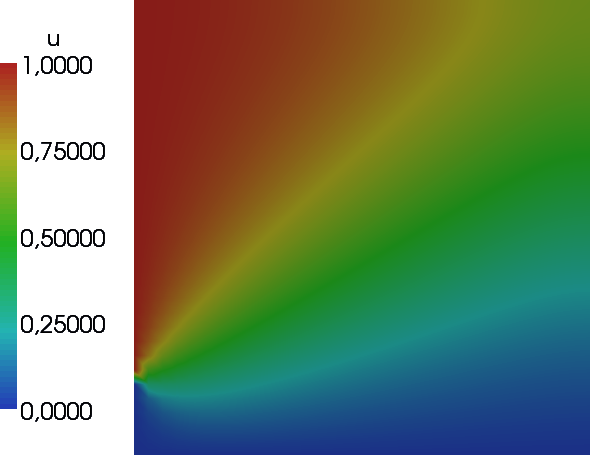
\includegraphics[width=0.45\textwidth]{fig/5_0,1.png}
\caption{The solution on a five times refined grid with $\nu = 0.1$.}
\label{reflevel5_nu0,1}
\end{center}
\end{figure}

\begin{figure}[htbp]
\begin{center}
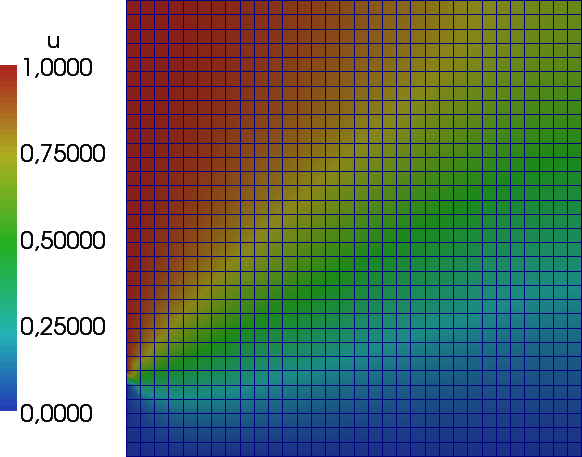
\includegraphics[width=0.45\textwidth]{fig/5_0,1_mit_Gitter.png}
\caption{The solution on a five times refined grid with $\nu = 0.1$ and its mesh.}
\label{}
\end{center}
\end{figure}

\begin{figure}[htbp]
\begin{center}
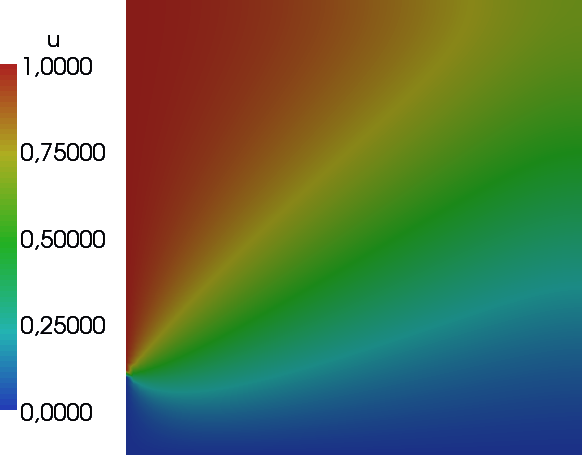
\includegraphics[width=0.45\textwidth]{fig/6_0,1.png}
\caption{The solution on a six times refined grid with $\nu = 0.1$.}
\label{reflevel6_nu0,1}
\end{center}
\end{figure}

For a numerical check of the theoretical results we used the above setup and varied the coefficient of diffusion $\nu$ and the fineness of the grid $h$. The following table shows the tested cases:
\newline
\begin{center}
\begin{tabular}{c|c|c|c|c|c|c}
\textbf{Level of refinement} & $h$ & $\nu$ & \textbf{P\'{e}clet number} & \textbf{stable}  & \textbf{Iterations} & \textbf{Figure} \\ \hline\hline
5 & 0.03125 & 0.1 & 0.15625 & yes  & 92 & \ref{reflevel5_nu0,1} \\
5 & 0.03125 & 0.025 & 0.625 & yes & 83 \\
5 & 0.03125 & 0.02 & 0.78125 & yes & 90 \\
5 & 0.03125 & 0.015 & 1.0416666667 & no & 92 & \ref{reflevel5_nu0,015} \\
5 & 0.03125 & 0.0015 & 10.4166666667 & no & 161 \\
5 & 0.03125 & 0.001 & 15.625 & no &  215 & \ref{reflevel5_nu0,001} \\ \hline
6 & 0.015625 & 0.1 & 0.078125 & yes & 275 \\
6 & 0.015625 & 0.02 & 0.390625 & yes & 313 \\
6 & 0.015625 & 0.01 & 0.78125 & yes & 359 \\
6 & 0.015625 & 0.007815 & 0.9996801024 & yes & 350 \\
6 & 0.015625 & 0.00625 & 1.25 & no & 387 & \ref{reflevel6_nu0,00625} \\
6 & 0.015625 & 0.005 & 1.5625 & no & 374 \\
6 & 0.015625 & 0.001 & 7.8125 & no & 400 \\
6 & 0.015625 & 0.0001 & 78.125 & no & 640 & \ref{reflevel6_nu0,0001}
\end{tabular}
\end{center}

For all tests the degree of the Lagrangian ansatz functions was one, i.e. we tested with linear elements.

\begin{figure}[htbp]
\begin{center}
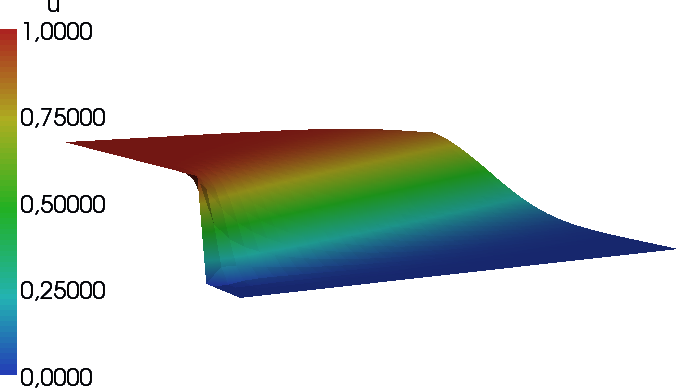
\includegraphics[width=0.55\textwidth]{fig/5_0,015_gedreht.png}
\caption{The solution on a five times refined grid with $\nu = 0.015$.}
\label{reflevel5_nu0,015}
\end{center}
\end{figure}

\begin{figure}[htbp]
\begin{center}
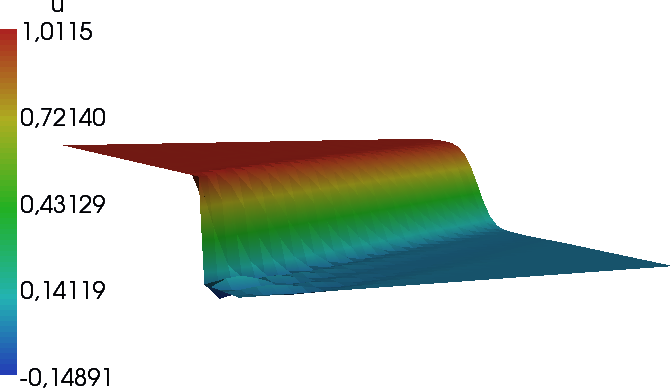
\includegraphics[width=0.55\textwidth]{fig/5_0,001_gedreht.png}
\caption{The solution on a five times refined grid with $\nu = 0.001$.}
\label{reflevel5_nu0,001}
\end{center}
\end{figure}

\begin{figure}[htbp]
\begin{center}
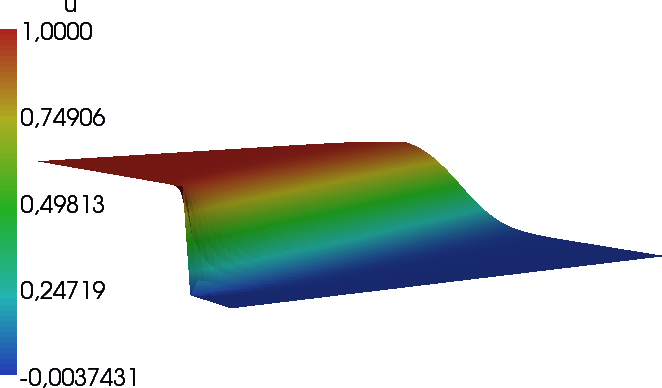
\includegraphics[width=0.55\textwidth]{fig/6_0,00625.png}
\caption{The solution on a six times refined grid with $\nu = 0.00625$.}
\label{reflevel6_nu0,00625}
\end{center}
\end{figure}

\begin{figure}[htbp]
\begin{center}
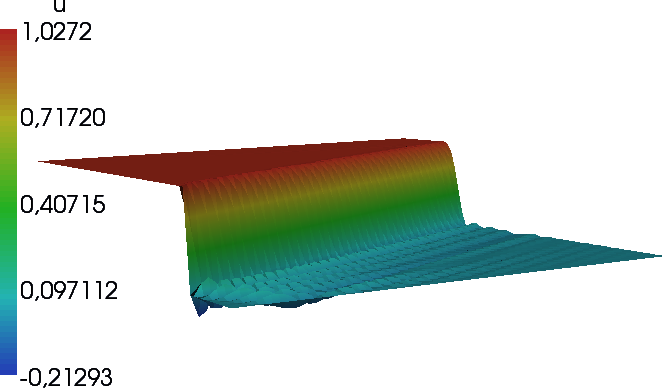
\includegraphics[width=0.55\textwidth]{fig/6_0,0001.png}
\caption{The solution on a six times refined grid with $\nu = 0.0001$.}
\label{reflevel6_nu0,0001}
\end{center}
\end{figure}

The results and the shown Figures clearly reflect the theoretical results about the stability. For $P_{e} \leq 1$ the solutions are stable and no oscillations occur. Interesting is the case of Figure \ref{reflevel5_nu0,015} where the P\'{e}clet number is slightly greater than one. The theory states that the solution is not stable any more, but in practice the oscillations are too small to be visible and also a direct analysis of the values at the nodes shows no obvious indications for them. But in Figure \ref{reflevel6_nu0,00625}, where $P_{e} = 1.25$, the oscillations are clearly visible and also of course for higher P\'{e}clet numbers.

So we can say that the theoretical results are quite sharp and are reflected by our practical examinations.

The question is now how we can stabilize the numerical solution process. As we mentioned above the number of unknowns increases exponentionally with the level of refinement and so further and further refinement of the grid to obtain a stable solution might not be feasible any more. Furthermore the diffusion $\nu$ can not be chosen freely in applications because it is fixed by the underlying physical problem.

So we will next discuss two stabilization schemes for the steady convection-diffusion problem.

\subsection{SUPG Method}

Writing out the stabilization term in \eqref{stabilization} with the weighting operator \eqref{SUPG} yields

	\[\left(R(u), \tau W(v)\right)_{h} = \tau(a \cdot \nabla u, a \cdot \nabla v)_{h} - \tau\nu(\Delta u, a \cdot \nabla v)_{h}.\]
	
The first term on the right hand side is the already mentioned artificial diffusion that is projected in the direction of the convection velocity $a$. So we can expect that the solution is smoothed in the direction of the convectivity while the structure of the solution reflects the physical parameters, especially the given diffusion.

That way we loose the constraints on $P_{e}$, see section \ref{comparison}.

We tested the SUPG method with the cases that turned out to be the most unstable in section \ref{sec:nostab}. The following table gives an overview of the obtained results:

\begin{center}
\begin{tabular}{c|c|c|c|c}
\textbf{Level of refinement} & $\nu$ & \textbf{P\'{e}clet number} & \textbf{Iterations (SUPG)} & \textbf{Figure} \\ \hline\hline
5 & 0.0015 & 10.4166666667	& 903 & \ref{SUPGreflevel5_nu0,0015}\\
5 & 0.001 & 15.625	& 881 & \ref{SUPGreflevel5_nu0,001} \\ \hline
6 & 0.001 & 7.8125	& 3150 & \ref{SUPGreflevel6_nu0,001} \\
6 & 0.0001 & 78.125 & 3121 & \ref{SUPGreflevel6_nu0,0001}
\end{tabular}
\end{center}

\begin{figure}[htbp]
\begin{center}
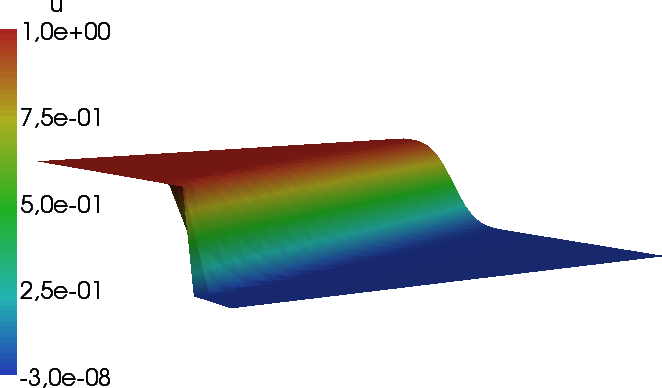
\includegraphics[width=0.55\textwidth]{fig/SUPG_5_0,0015_quad.png}
\caption{The solution on a five times refined grid with $\nu = 0.0015$ stabilized with the SUPG method with quadratic elements.}
\label{SUPGreflevel5_nu0,0015}
\end{center}
\end{figure}

\begin{figure}[htbp]
\begin{center}
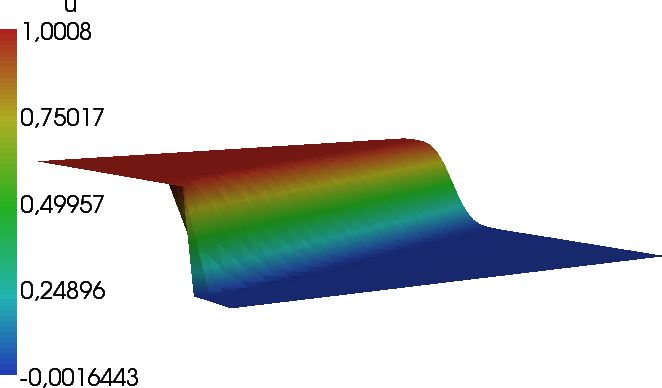
\includegraphics[width=0.55\textwidth]{fig/SUPG_5_0,001_quad.png}
\caption{The solution on a five times refined grid with $\nu = 0.001$ stabilized with the SUPG method with quadratic elements.}
\label{SUPGreflevel5_nu0,001}
\end{center}
\end{figure}

\begin{figure}[htbp]
\begin{center}
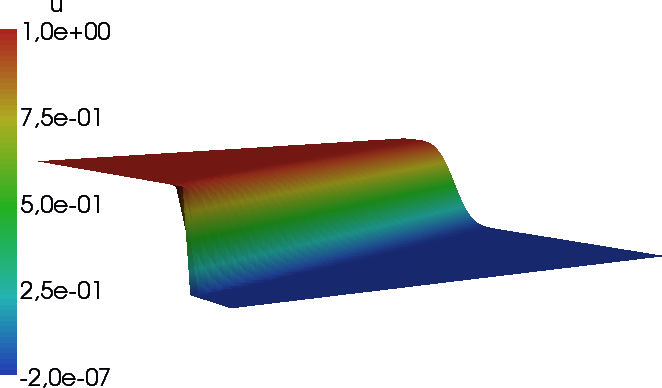
\includegraphics[width=0.55\textwidth]{fig/SUPG_6_0,001_quad.png}
\caption{The solution on a six times refined grid with $\nu = 0.001$ stabilized with the SUPG method with quadratic elements.}
\label{SUPGreflevel6_nu0,001}
\end{center}
\end{figure}

\begin{figure}[htbp]
\begin{center}
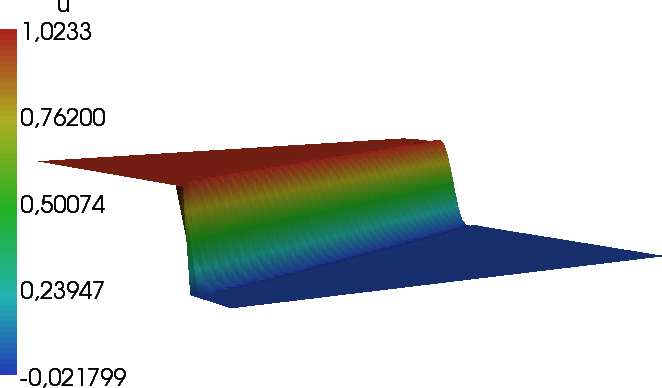
\includegraphics[width=0.55\textwidth]{fig/SUPG_6_0,0001_quad.png}
\caption{The solution on a six times refined grid with $\nu = 0.0001$ stabilized with the SUPG method with quadratic elements.}
\label{SUPGreflevel6_nu0,0001}
\end{center}
\end{figure}

As the Figures show the SUPG method does not miss its target. All computed solutions do show much less oscillations and are stable but the oscillations are only damped and do not vanish. Nonetheless the quality of the approximation is quite good. The tests also show that the often proposed choice of $\tau$ from section \ref{parameter} is a not too bad choice for it leads to approximations of good quality because they show qualitatively the behaviour that we expect analytically.


\subsection{GLS Method}

An issue in the SUPG method is the added stabilization term, which is not symmetric in $u$ and $v$ and thus makes it difficult to establish statements on the stability. The GLS methos avoids this problem as we will see now.

Writing out the stabilization term in \eqref{stabilization} with the weighting operator \eqref{GLS} yields

	\[\left(R(u), \tau W(v)\right)_{h} = \tau(a \cdot \nabla u, a \cdot \nabla v)_{h} - \tau\nu(\Delta u, a \cdot \nabla v)_{h} - \tau\nu(a \cdot \nabla u, \Delta v)_{h} + \tau\nu^{2}(\Delta u, \Delta v)_{h}.\]
	
The first term on the right hand side is the already mentioned artificial diffusion that is projected in the direction of the convection velocity $a$.

For linear ansatz function the SUPG and the GLS method coincide. That is the reason why we chose quadratic ansatz functions for our tests because then we expect to obtain some differences between the two methods.

As with the SUPG method, we tested the GLS method with the cases that turned out to be the most unstable in section \ref{numeric}. The following table gives an overview of the obtained results:

\begin{center}
\begin{tabular}{c|c|c|c|c}
\textbf{Level of refinement} & $\nu$ & \textbf{P\'{e}clet number} & \textbf{Iterations (GLS)} & \textbf{Figure} \\ \hline\hline
5 & 0.0015 & 10.4166666667	& 845 & \ref{GLSreflevel5_nu0,0015} \\
5 & 0.001 & 15.625	& 830 & \ref{GLSreflevel5_nu0,001} \\ \hline
6 & 0.001 & 7.8125	& 1958 & \ref{GLSreflevel6_nu0,001} \\
6 & 0.0001 & 78.125 & 2898 & \ref{GLSreflevel6_nu0,0001}
\end{tabular}
\end{center}

\begin{figure}[htbp]
\begin{center}
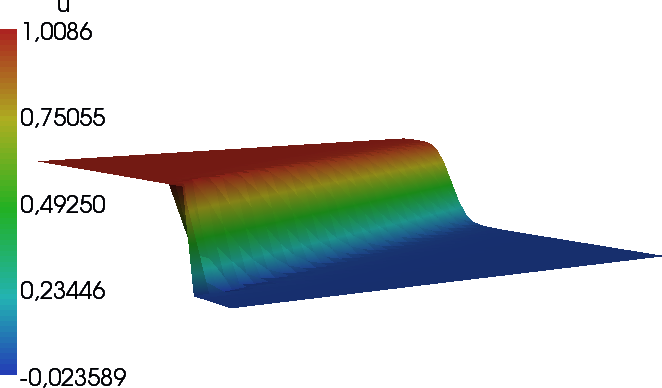
\includegraphics[width=0.55\textwidth]{fig/GLS_5_0,0015.png}
\caption{The solution on a five times refined grid with $\nu = 0.0015$ stabilized with the GLS method with quadratic elements.}
\label{GLSreflevel5_nu0,0015}
\end{center}
\end{figure}

\begin{figure}[htbp]
\begin{center}
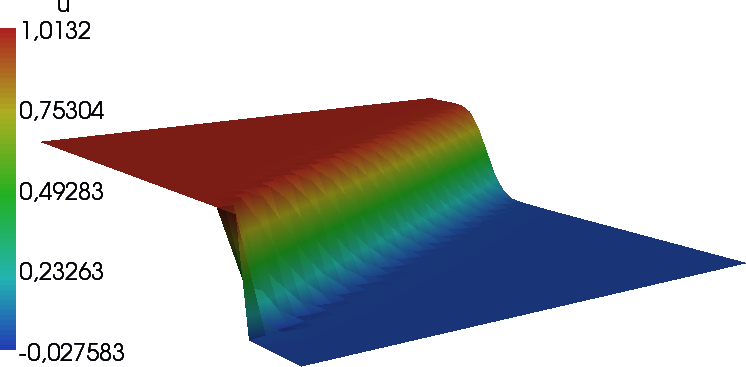
\includegraphics[width=0.55\textwidth]{fig/GLS_5_0,001_quad.png}
\caption{The solution on a five times refined grid with $\nu = 0.001$ stabilized with the GLS method with quadratic elements.}
\label{GLSreflevel5_nu0,001}
\end{center}
\end{figure}

\begin{figure}[htbp]
\begin{center}
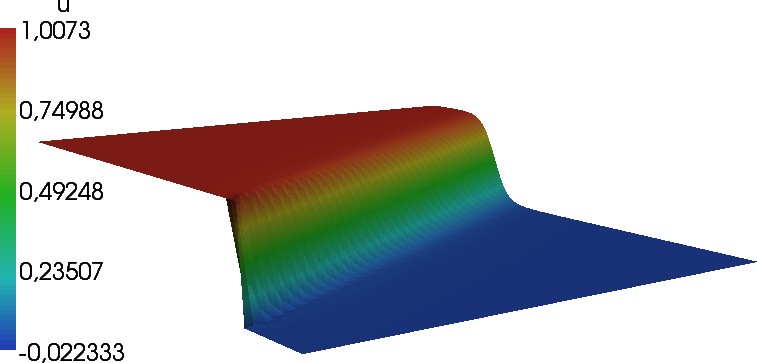
\includegraphics[width=0.55\textwidth]{fig/GLS_6_0,001_quad.png}
\caption{The solution on a six times refined grid with $\nu = 0.001$ stabilized with the GLS method with quadratic elements.}
\label{GLSreflevel6_nu0,001}
\end{center}
\end{figure}

\begin{figure}[htbp]
\begin{center}
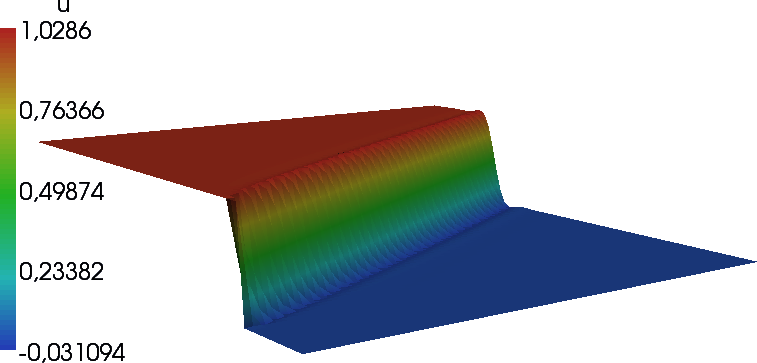
\includegraphics[width=0.55\textwidth]{fig/GLS_6_0,0001_quad.png}
\caption{The solution on a six times refined grid with $\nu = 0.0001$ stabilized with the GLS method with quadratic elements.}
\label{GLSreflevel6_nu0,0001}
\end{center}
\end{figure}

Also so GLS method does not miss its target and produces stable solutions. But a direct comparison of the SUPG and the GLS methods shows that the quality of the approximation is better with the SUPG method because the oscillations are damped a little bit better than with the GLS method.

\subsection{Comparison of the Two Stabilization Methods}\label{comparison}

First, we want to mention that the stability of both methods can be proved under certain assumptions, see e.g. \cite{Quarteroni}. It even turns out that we loose the constraints on $P_{e}$ and obtain constraints on $h$ and $\tau$ that are linked and depend on $P_{e}$. So the problem are not the parameters of the underlying physical problem any more but the right choice of the parameters of the numerical approximation. The additional parameter $\tau$ allows us to choose $h$ so large that the numerical computation of the solution is feasible.

The differences in the difficulty and complexity of the implementation are marginal because only the assembling of the system matrix has to be modified for the GLS method, i.e. the two additional terms have to be implemented.

A little drawback of the SUPG method is the efficiency compared to the GLS method because as the above results show the SUPG method needs more iterations in the GMRES solver algorithm than the GLS method. But the differences are not big enough to abolish the SUPG method because they only differ about $10 \%$.

\newpage
\appendix
\bibliography{tutorials_bib}
\bibliographystyle{plain}

\printindex

\end{document}
